%
% schichtung.tex -- Tiefenaufbau des Meeres
%
% (c) 2018 Prof Dr Andreas Müller, Hochschule Rapperswil
%
\section{Aufbau der Meere\label{section:thc:schichtung}}
\rhead{Aufbau der Meere}
\begin{figure}
\centering
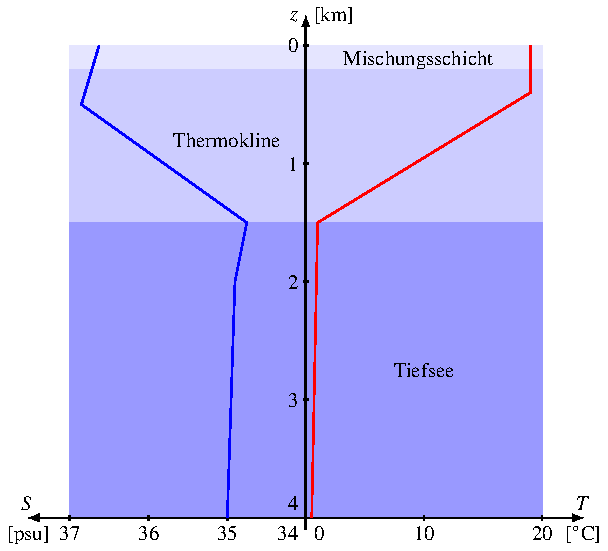
\includegraphics{chapters/4/schichten.pdf}
\caption{Tiefenaufbau des Meeres mit schematischem
Temperatur- und Salinitätsprofil.
Die Richtung der Achsen ist so gewählt, dass ``rechts'' gleichbedeutend
ist mit höher Dichte.
\label{skript:thc:schichtung}}
\end{figure}
Die Weltmeere umfassen etwa 1.4 Milliarden $\text{km}^3$ Wasser.
Wegen der hohen Wärmekapazität von $4.182\,\text{kJ}/\text{kg}\cdot\text{K}$
ist dies ein gigantisches Wärmereservoir mit entsprechend grosser
Bedeutung für das Klima.
Für das Verständnis des Klimassystems der Erde ist also die Kenntnis
des Aufbaus der Meere sowie des Energietransports in den Meeren unabdingbar.

Eine Reihe von Mechanismen beeinflussen Temperatur und Salinität.
An der Oberfläche wärmt sich das Wasser durch Einstrahlung
oder Zufluss warmen Wassers auf.
Wärmeaustausch mit der Atmosphäre gleicht die Temperatur von
Meer und Atmosphäre an, Verdunstung benötigt Energie und kühlt das Meer ab.
Der Zufluss von Süsswasser reduziert den Salzgehalt, die Verdungstung erhöht
die Salzkonzentration.
Durch Wind angeregte Turbulenz sorgt für gute Durchmischung dieser 
sogenannten {\em Mischungsschicht},
\index{Mischungsschicht}%
in ihr sind Temperatur und Salinität daher ungefähr konstant.
Sie reicht bis in eine Tiefe von wenigen hundert Metern.

In der Tiefe stehen bis auf einzelne wenige Stellen keine Quellen oder
Senken von Wärme oder Salz zur Verfügung.
Dort fehlt damit auch der Antrieb für Umwälzbewegungen, es bleibt
nur die Diffusion und die Schwerkraft.
Man kann daher davon ausgehen, dass in grosser Tiefe kaltes Wasser 
liegt mit weitgehend konstanter Temperatur und konstantem Salzgehalt.
Dies ist die {\em Tiefsee}.
\index{Tiefsee}%

Zwischen der Mischungsschicht und dem Tiefenwasser findet ein Ausgleich
von Temperatur und Salzgehalt statt.
Da dieser Ausgleich umso schneller erfolgt, je grösser der Unterschied
von Temperatur und Salinität erfolgt, ist ein Fliessgleichgewicht nur
möglich, wenn Temperatur und und Salinität in dieser Zone linear
von der Tiefe abhängen.
Diesen Bereich nennt man die {\em Thermokline}.
\index{Thermokline}%
Fehlt die Thermokline, hat das Oberflächenwasser die gleichen Eigenschaften
wie das Tiefenwasser, insbesondere gibt es keine Unterschiede, die eine
Umwälzung im Meer herbeiführen würden.
Je grösser tie Thermoklinentiefe, desto grösser auch der Unterschied
zwischen Obeflächenwasser und Tiefenwasser und desto mehr Energie für
den Antrieb der Zirkulation ist im Meer gespeichert.

